% The angle group Z/8: the +1 cycle and the doubling endomorphism k -> 2k.
\documentclass[tikz,border=8pt]{standalone}
\usepackage{amsmath,amssymb}
\usetikzlibrary{arrows.meta}
\begin{document}
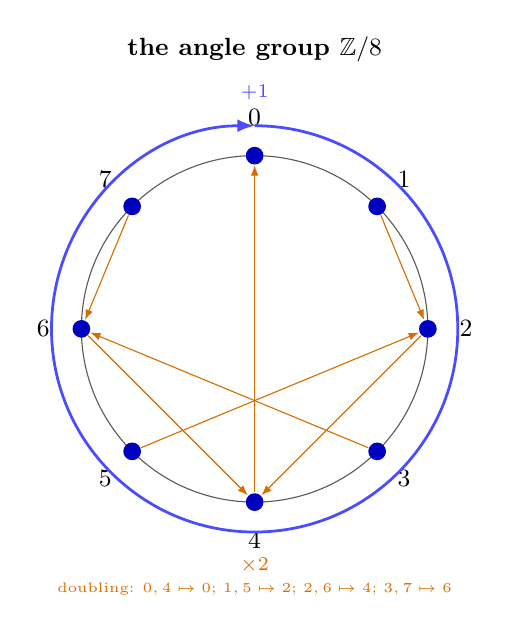
\begin{tikzpicture}[scale=1.0]
  \def\R{2.2}
  \draw[black!65] (0,0) circle (\R);
  \foreach \k in {0,...,7} {%
    \pgfmathsetmacro{\ang}{90-45*\k}%
    \coordinate (A\k) at (\ang:\R);%
    \fill[blue!75!black] (A\k) circle (3.2pt);%
    \node[font=\small] at (\ang:1.22*\R) {\k};%
  }
  % +1 cycle: one full turn
  \draw[-{Latex[length=2.2mm]}, blue!70, line width=1pt]
    (0,\R+0.38) arc (90:-270:\R+0.38);
  \node[font=\scriptsize,text=blue!70] at (0,3.0) {$+1$};
  % doubling chords k -> 2k
  \foreach \a/\b in {1/2,2/4,4/0,3/6,6/4,5/2,7/6} {%
    \draw[-{Latex[length=1.3mm]}, orange!85!black,
          shorten >=3.5pt, shorten <=3.5pt] (A\a) -- (A\b);}
  \node[font=\scriptsize,text=orange!85!black] at (0,-3.0) {$\times 2$};
  \node[font=\small\bfseries] at (0,3.55) {the angle group $\mathbb Z/8$};
  \node[font=\tiny,text=orange!85!black] at (0,-3.3) {doubling: $0,4\mapsto0$; $1,5\mapsto2$; $2,6\mapsto4$; $3,7\mapsto6$};
\end{tikzpicture}
\end{document}
